\section{ALGORITHM\textbackslash METHODOLOGY}
\noindent\uline{Five types of Platonic Solids}: 
\begin{figure}[h]
\centering
	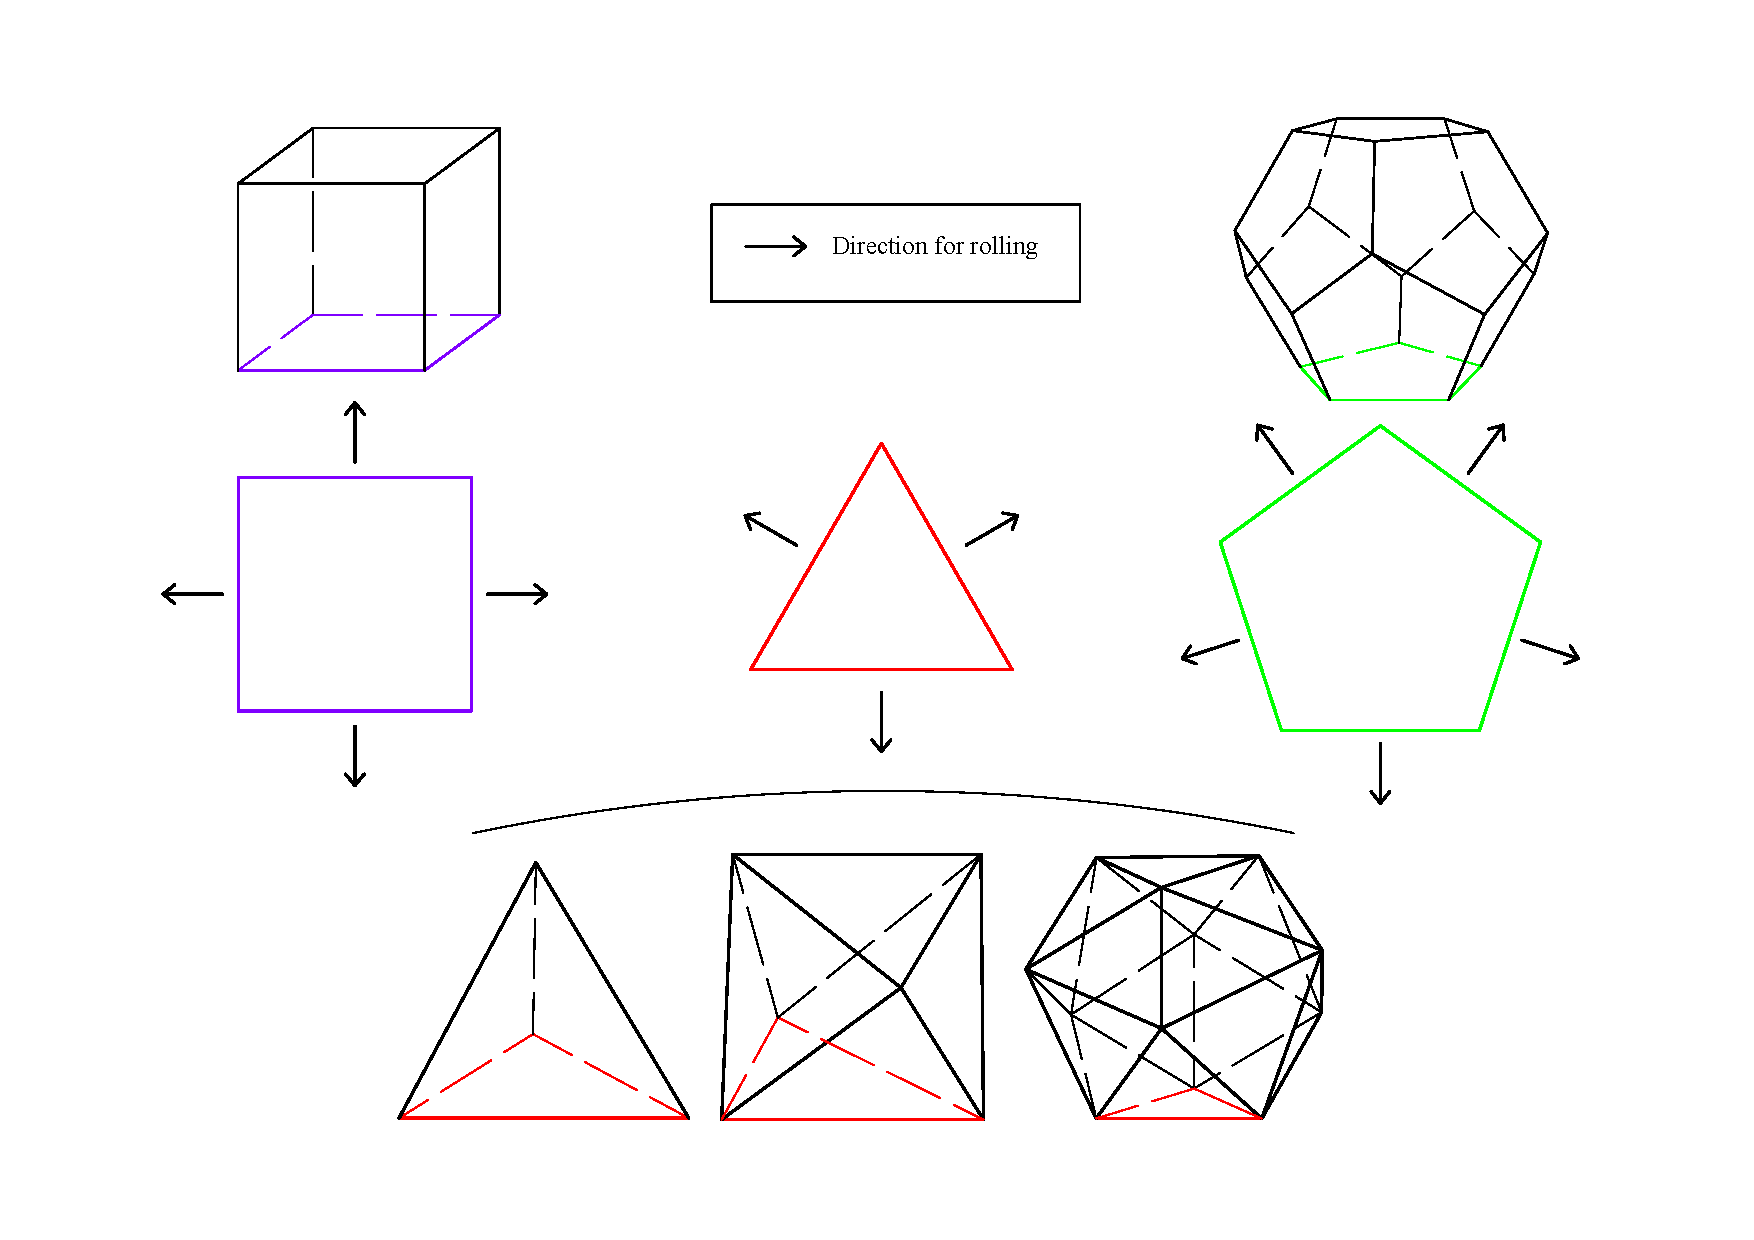
\includegraphics[width=1\textwidth]{image/rollingDir2.pdf}
	\caption{Rolling direction for each types of platonic solids}
	\label{fig:platonicSolids}
\end{figure}\\
%
% 
%
%
%
%
%
\uline{Version1}: \\

Example:\\
\begin{algorithm}[H]
\SetAlgoLined
\KwResult{\textit{Write here the result }}
 initialization\;
 \While{While condition}{
  instructions\;
  \eIf{condition}{
   instructions1\;
   instructions2\;
   }{
   instructions3\;
  }
 }
 \caption{How to write algorithms}
\end{algorithm}


\noindent\uline{Version2}: 
% algorithm code (for this example)
\begin{algorithm}

% functions
\SetKwFunction{cumprod}{cumprod}
\SetKwFunction{length}{length}
\SetKwFunction{zeros}{zeros}
\SetKwFunction{ceil}{ceil}

% input/ouput names
\SetKwInOut{Input}{Input}
\SetKwInOut{Output}{Output}

% caption
\caption{Creation of edge set for a specific perfect matching number.\label{alg:singlepm}}

\Input{%
		\xvbox{2mm}{$\xvar{N}$} -- number of vertices (should be even) \\
		\xvbox{2mm}{$\xvar{I}$} -- perfect matching number, integer between 1 and $(\xvar{N}-1)!!$
	  }
\Output{%
		\xvbox{2mm}{$\xvar{E}$} -- vector of edges in sequential pairs
	   }

  \BlankLine % blank line for spacing
  
  % start of the pseudocode
  \xvbox{2mm}{$\xvar{J}$} $\leftarrow$ $[ 1,3,5,\dots,\xvar{N}-1 ]$ \tcc*{odd numbers from 1 to N-1}

  \xvbox{2mm}{$\xvar{P}$} $\leftarrow$ $[ 1,\cumprod(\xvar{J}) ]$ \tcc*{cumulative double factorial}
    
  \xvbox{2mm}{$\xvar{V}$} $\leftarrow$ $[ 1,2,\dots,\xvar{N} ]$ \tcc*{create initial list of available vertices}
        
  \For{$\xvar{j}\leftarrow$ $\xvar{J}$ }{

    \xvbox{1mm}{$\xvar{q}$} $\leftarrow$ $(\xvar{N}+1-\xvar{j})/2$ \tcc*{index for 2nd to last entry in P}

    \xvbox{1mm}{$\xvar{I}$} $\leftarrow$ $\ceil\big(\xvar{I}/\xvar{P}(\xvar{q})\big)$ \tcc*{calculate smaller vertex index}

    $\xvar{E}(\xvar{j})$ $\leftarrow$ $\xvar{V}(\xvar{end})$ \tcc*{assign largest remaining value}

    remove element $\xvar{V}(\xvar{end})$ \tcc*{remove largest remaining value}

    $\xvar{E}(\xvar{j}+1)$ $\leftarrow$ $\xvar{V}(\xvar{i})$ \tcc*{assign smaller selected value}

    remove element $\xvar{V}(\xvar{i})$ \tcc*{remove the smaller selected value}

    \xvbox{1mm}{$\xvar{I}$} $\leftarrow$ $\xvar{I} - \big( (\xvar{i} - 1) \times \xvar{P} (\xvar{q}) \big)$ \tcc*{subtract to get index in subgraph with 2 vertices removed}
	
  } % end for j	

\end{algorithm}
\clearpage
\newpage